%%%%%%%%%%%%%%%%%%%%%%%%%%%%%%%%%%%%%%
%% Frame
%%%%%%%%%%%%%%%%%%%%%%%%%%%%%%%%%%%%%%

\begin{frame}[t]
\frametitle{Incoherence}
\framesubtitle{~~}  %% needed for proper positioning of the logo ...

Recall that the incoherence of two matrices $\Phi$ and $\Psi$ is given by 

\begin{align}
	\mu = \max_{i,j} |(\Phi \Psi)_{ij}|
	\label{incoherence}
\end{align}

Why is incoherence important?

\begin{itemize}
	\item More incoherence $\implies$ more chance at ``catching'' sparsity
	\item Less incoherence $\implies$ more measurements needed
	\item Plays an important role in recovery proofs due to Candes and Romberg (2007)
	\item We did an experiment to demonstrate the importance of incoherence
\end{itemize}
\end{frame}

%%%%%%%%%%%%%%%%%%%%%%%%%%%%%%%%%%%%%%
%% Frame
%%%%%%%%%%%%%%%%%%%%%%%%%%%%%%%%%%%%%%
\begin{frame}[t]
\frametitle{Incoherence}
\framesubtitle{~~}  %% needed for proper positioning of the logo ...

\begin{figure}[h!]
  \centering
    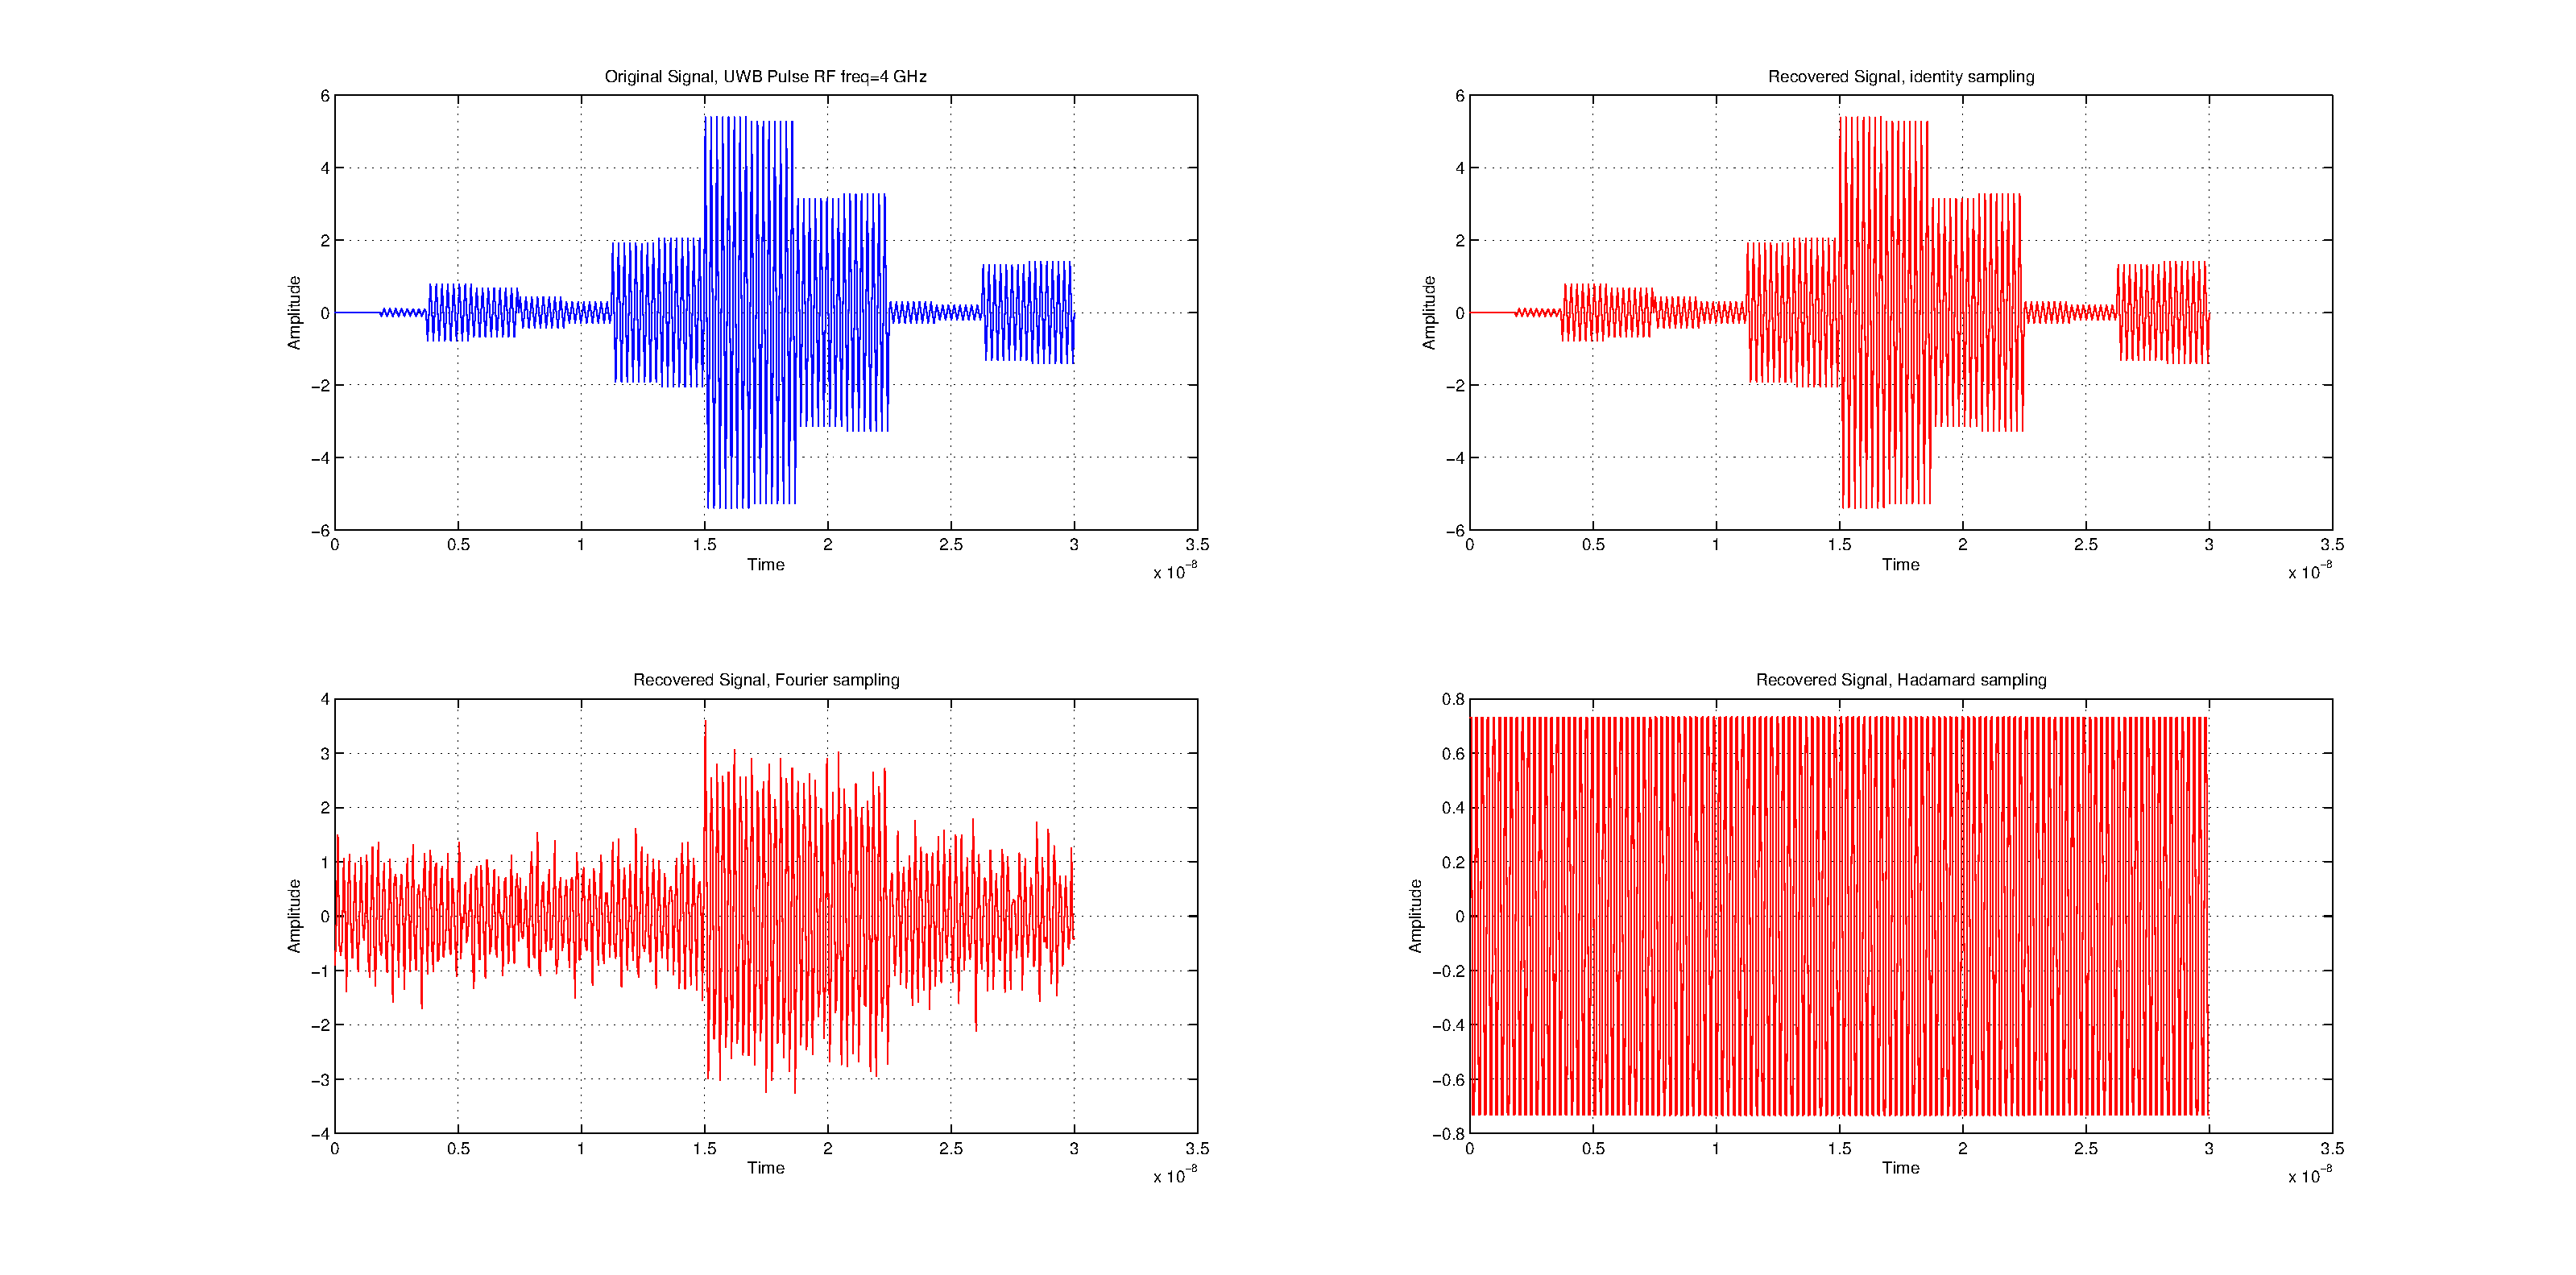
\includegraphics[width=1\textwidth]{figs/incoherence.pdf}
\end{figure}


\end{frame}

%%%%%%%%%%%%%%%%%%%%%%%%%%%%%%%%%%%%%%
%% Frame
%%%%%%%%%%%%%%%%%%%%%%%%%%%%%%%%%%%%%%
\begin{frame}[t]
\frametitle{Incoherence}
\framesubtitle{~~}  %% needed for proper positioning of the logo ...

From Romberg (2008), we have the result:\\

\textbf{Lemma 3.1:} \textit{Let $\boldsymbol{\Phi}$ be an arbitrary fixed orthogonal matrix
, and create $H$ at random with $H = N^{-\frac{1}{2}} F^* \Sigma F$. Choose $0<\delta<1$.
Then with probability exceeding $1-\delta$, the coherence $\mu(H,\boldsymbol{\Phi})$ 
will obey} \\
\begin{equation}
	\mu(H,\boldsymbol{\Phi}) \leq 2 \sqrt{\log \left(\frac{2N^2}{\delta} \right)}
	\label{incoherence_bd1}
\end{equation}
\\
Our random basis is incoherent to \textbf{any} basis with a high probability!

\end{frame}



%%%%%%%%%%%%%%%%%%%%%%%%%%%%%%%%%%%%%%
%% Frame
%%%%%%%%%%%%%%%%%%%%%%%%%%%%%%%%%%%%%%
\begin{frame}[t]
\frametitle{Incoherence}
\framesubtitle{~~}  %% needed for proper positioning of the logo ...

From Do et al (2012), we have the result:\\

\textbf{Theorem III.3:} \textit{Given $F$ and $R$ as defined above, let $A=FR$, and $\Phi$ a fixed orthogonal matrix. Then if the magnitude of the entries of $F$ are bounded by $\mathcal{O}(\frac{1}{\sqrt{B}})$, we have that}
\begin{equation}
	\mu(A,\Phi) \leq \mathcal{O}\left(\sqrt{\frac{\log{\frac{N}{\delta}}}{B}}\right)
\end{equation}
Additionally, if the maximal entry of $\Phi$ (the sparsity domain) is $\mathcal{O}\left(\frac{1}{\sqrt{N}}\right)$,
we can change the bound to 
\begin{equation}
	\label{incoherence_bd2}
	\mu(A,\Phi) \leq \mathcal{O} \left( \sqrt{\frac{\log{\frac{N}{\delta}}}{N}}\right)
\end{equation}

\end{frame}
